\section{Electronics and Light Monitoring System}

\subsection{Electronics}

The electronics of the HTCC provides spectrometric and timing information for electron scattering events that
are detected by the HTCC within its acceptance. Two fast output signals are required from each channel in order
to generate a fast trigger for the CLAS12 spectrometer~\cite{trigger-nim}. This required that the anode signal
from the PMT had to be split or that the voltage divider for the PMT be modified by adding a fast preamplifier to
generate two identical signals with the same polarity. In our case we have chosen to use a modified standard linear
passive high voltage divider that is equipped with a fast preamplifier, see Fig.~\ref{fig:POPOV_1}. This preamplifier
is integrated in the original divider and does not need external power supplies other than the same high voltage
power supply used for the PMTs. The amplification coefficient varies from 8 to 10. The preamplifier provides two
output signals of negative polarity. 

\begin{figure}[!ht]
    \centering
    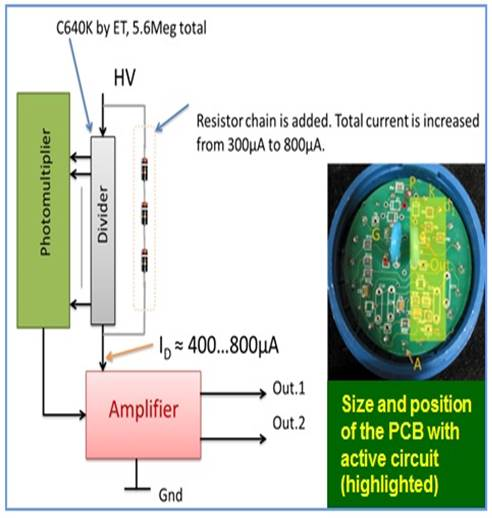
\includegraphics[width=1.0\linewidth,trim={0.0cm 0.0cm 0.0cm 0.0cm},clip]{images/POPOV_1.jpg}
    \caption{Modified high voltage divider with 2 identical outputs used for the HTCC.}
    \label{fig:POPOV_1}
\end{figure}

The preamplifier is also fast: the signal rise time increases by 1.5~ns as compared with signal from a passive divider,
and it is almost as fast as a signal from fast plastic scintillators. Figs.~\ref{fig:POPOV_2} and \ref{fig:POPOV_3}
show typical signals provided by a standard passive divider and by the modified divider, respectively. The pulses
have near perfect output termination with no signs of any ringing or after-pulsing.

\begin{figure}[!ht]
    \centering
    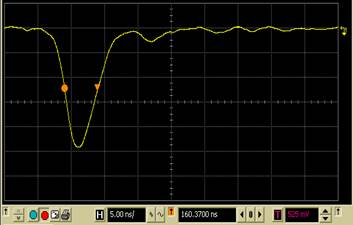
\includegraphics[width=1.0\linewidth,trim={0.0cm 0.0cm 0.0cm 0.0cm},clip]{images/POPOV_2.jpg}
    \caption{Typical output signal provided by passive HV-divider.}
    \label{fig:POPOV_2}
\end{figure}

\begin{figure}[!ht]
    \centering
    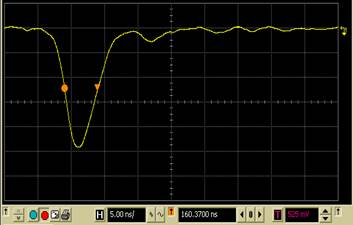
\includegraphics[width=1.0\linewidth,trim={0.0cm 0.0cm 0.0cm 0.0cm},clip]{images/POPOV_3.jpg}
    \caption{Typical output signal provided by the modified HV-divider with 2 identical outputs.}
    \label{fig:POPOV_3}
\end{figure}

The preamplifier is compact and reliable, and does not require any changes in the high voltage power supply or
in the cabling/connection scheme. It consumes relatively low current and does not need additional cooling.
 
It has to be mentioned that the preamplifier we use generates  additional noise as any other preamplifier
unavoidably would. However, we use 5-in photomultiplier tubes that have a large quartz face-plate. Even after
selecting PMTs with the lowest possible dark noise and using a standard linear passive divider designed for the
detection of low amplitude signals, it was impossible to observe any indication of a single photoelectron peak because
the PMTs were too noisy. Fig.~\ref{fig:POPOV_4} shows the calibration results for a representative PMT with a
modified divider.   

%\begin{comment}
% Measurements of the dark noise were obtained after we developed and used a special dark current measurement
% procedure that would not require any modification of the standard passive divider. It was important that we were
% able to avoid using any Nano-Ampere Meters because these meters would necessitate certain modifications to the
% dividers using positive high voltage. This process allows us to avoid using any meters, and to consequently avoid any
% changes. Instead of using meters we analyze the dark pulse spectra from the flash ADC, which is triggered by pulse
% generator. Thus the ratio of integrating the charge to the width of the time window when the charge was obtained
% provides an accurate and stable estimate of the dark current.
%\end{comment}

\begin{figure}[!ht]
    \centering
    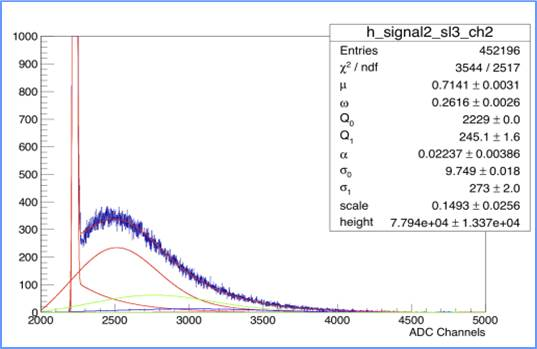
\includegraphics[width=1.0\linewidth,trim={0.0cm 0.0cm 0.0cm 0.0cm},clip]{images/POPOV_4.jpg}
    \caption{Calibration results for a representative PMT with a modified divider. The red curves represent a pedestal
      signal (narrow) and a single photoelectron peak. In the most cases PMTs have been used at high voltages lower (by
      about 600~V) than specified for the standard divider.}
    \label{fig:POPOV_4}
\end{figure}

\subsection{Light Monitoring System and Signal Readout}

In order to gain match phototubes that do not directly reveal the single photoelectron signal, we developed a new
external very fast light source with Light Emitting Diodes (LED). Fig.~\ref{fig:LMS_Picture_3} shows all
components of the HTCC Light Monitoring System (LMS). The device is remotely driven, allows for changes in the
emitted light intensity, and works at different frequencies in a wide range of these parameters. Once turned on,
and after temperature equilibrium is reached, the source is very stable in providing light signals with the required
strength and timing. There is an LED panel installed at the entry window of a 4-in diameter integrating sphere. This
panel illuminates the sphere and the light is distributed evenly between fifty coated clear fiber optics that are 1~mm
in diameter that form a bundle. All the fibers in the bundle have the same length and shine the light directly onto the
face of the PMT. The average light intensity is monitored and kept very stable during the entire period of
measurements. The average amplitude was at the level of a few photoelectrons. Since it is possible to adjust the
frequency of the light pulses, we were able to observe PMT signals that were well separated from the dark noise.
 
\begin{figure}[!ht]
    \centering
    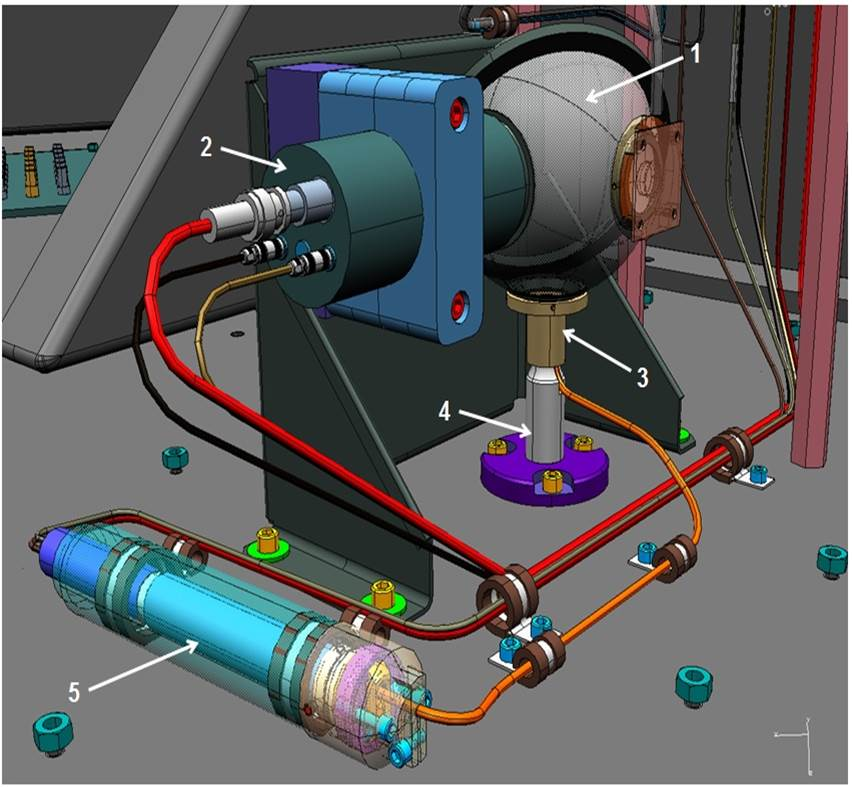
\includegraphics[width=1.0\linewidth,trim={0.0cm 0.0cm 0.0cm 0.0cm},clip]{images/LMS_Picture_3.jpg}
    \caption{The Light Monitoring System consists of an integrating sphere (1), fast light source (2), adapter (3),
      50 fiber optic cables bundled in a harness (4), and the reference PMT (5).}
    \label{fig:LMS_Picture_3}
\end{figure} 
 
The valuable features of the LMS and of the procedure for gain matching the phototubes are:
 
 \begin{itemize}
     \item The system can be used to calibrate either low-noise or high-noise PMTs;
     \item The LMS generated calibration light intensity was kept stable during data taking;
     \item It is only necessary to have the fiber optics deliver light intensity to all channels with 10-20\% uniformity;
     \item The calibration results are reproducible even if one uses different settings for the LED source;
     \item Maintenance of the LMS is essentially simplified since calibration of the LMS itself is not needed;
     \item Possible usage of the LMS as often as needed without the necessity of providing the same intensity of light
       source in different calibration sessions.
 \end{itemize}

The typical frequency of the LED light pulses is in the range of 6 to 10 kHz and is defined by a standard pulse
generator. The results obtained during the CLAS12 commissioning run and the following physics run with an
electron beam have shown that the information provided by JLab proprietary FADC250 modules (Flash ADC)
\cite{daq-nim} on HTCC signal strength and timing is sufficient. 

%\begin{comment}
%  No TDCs are used for the HTCC to get timing information. In other words, using just one output signal (without splitting)
%  would be preferable as opposed to the current option where an active high voltage divider provides two identical output
%  signals. One benefit of switching from active to passive dividers would be that one will be dealing with simplified and
%  therefore more reliable high voltage divider. Another valuable benefit would be also a certain reduction of noise in the
%  channels because no more preamplifiers would be in use. We plan to implement corresponding changes. Preliminary
%  comparative tests of two different dividers and same PMT show that the changes will provide higher quality results.
%\end{comment}
